\documentclass[../PS6_RapportFinal.tex]{subfiles}

\begin{document}
\graphicspath{{img/}{tex/img/}}

\thispagestyle{empty}
\enlargethispage{1cm}\vspace*{-2cm}
\begin{center}\normalfont\bfseries


\noindent\hspace*{-2.5cm}\includegraphics[height=2.2cm]{/logo/Logo_Saphire}

\par\vspace{.25cm}  Sciences Appliquées en Physique et Ingénierie  \par pour la Recherche et l'Enseignement\\
  \rule{\linewidth}{.25mm}


\par\vspace{1cm}  \textnormal{\bfseries RAPPORT DE PROJET PLURIDISCIPLINAIRE}

\par\vspace{.25cm} %\textnormal{effectué à "Nom de la structure d'accueil"}
\par\textnormal{sous la direction de Claire Limoge, Pierre Mella et Édouard Walther}
%\par\vspace{.25cm}\includegraphics[height=1.6cm]{/logo/LogoStage}


\par\vspace{\stretch{0.5}} \textnormal{\bfseries\huge PowerCompost 2.0}
\par\vspace{.5cm} {\bfseries par}
\par\vspace{.5cm}\textnormal{\bfseries\Large Ulysse Arliguié, Florentin Delaine, Antoine Fabre, Amal Fethi, Nicolas Muller et Richard Verwaerde}
\par\vspace{\stretch{0.5}}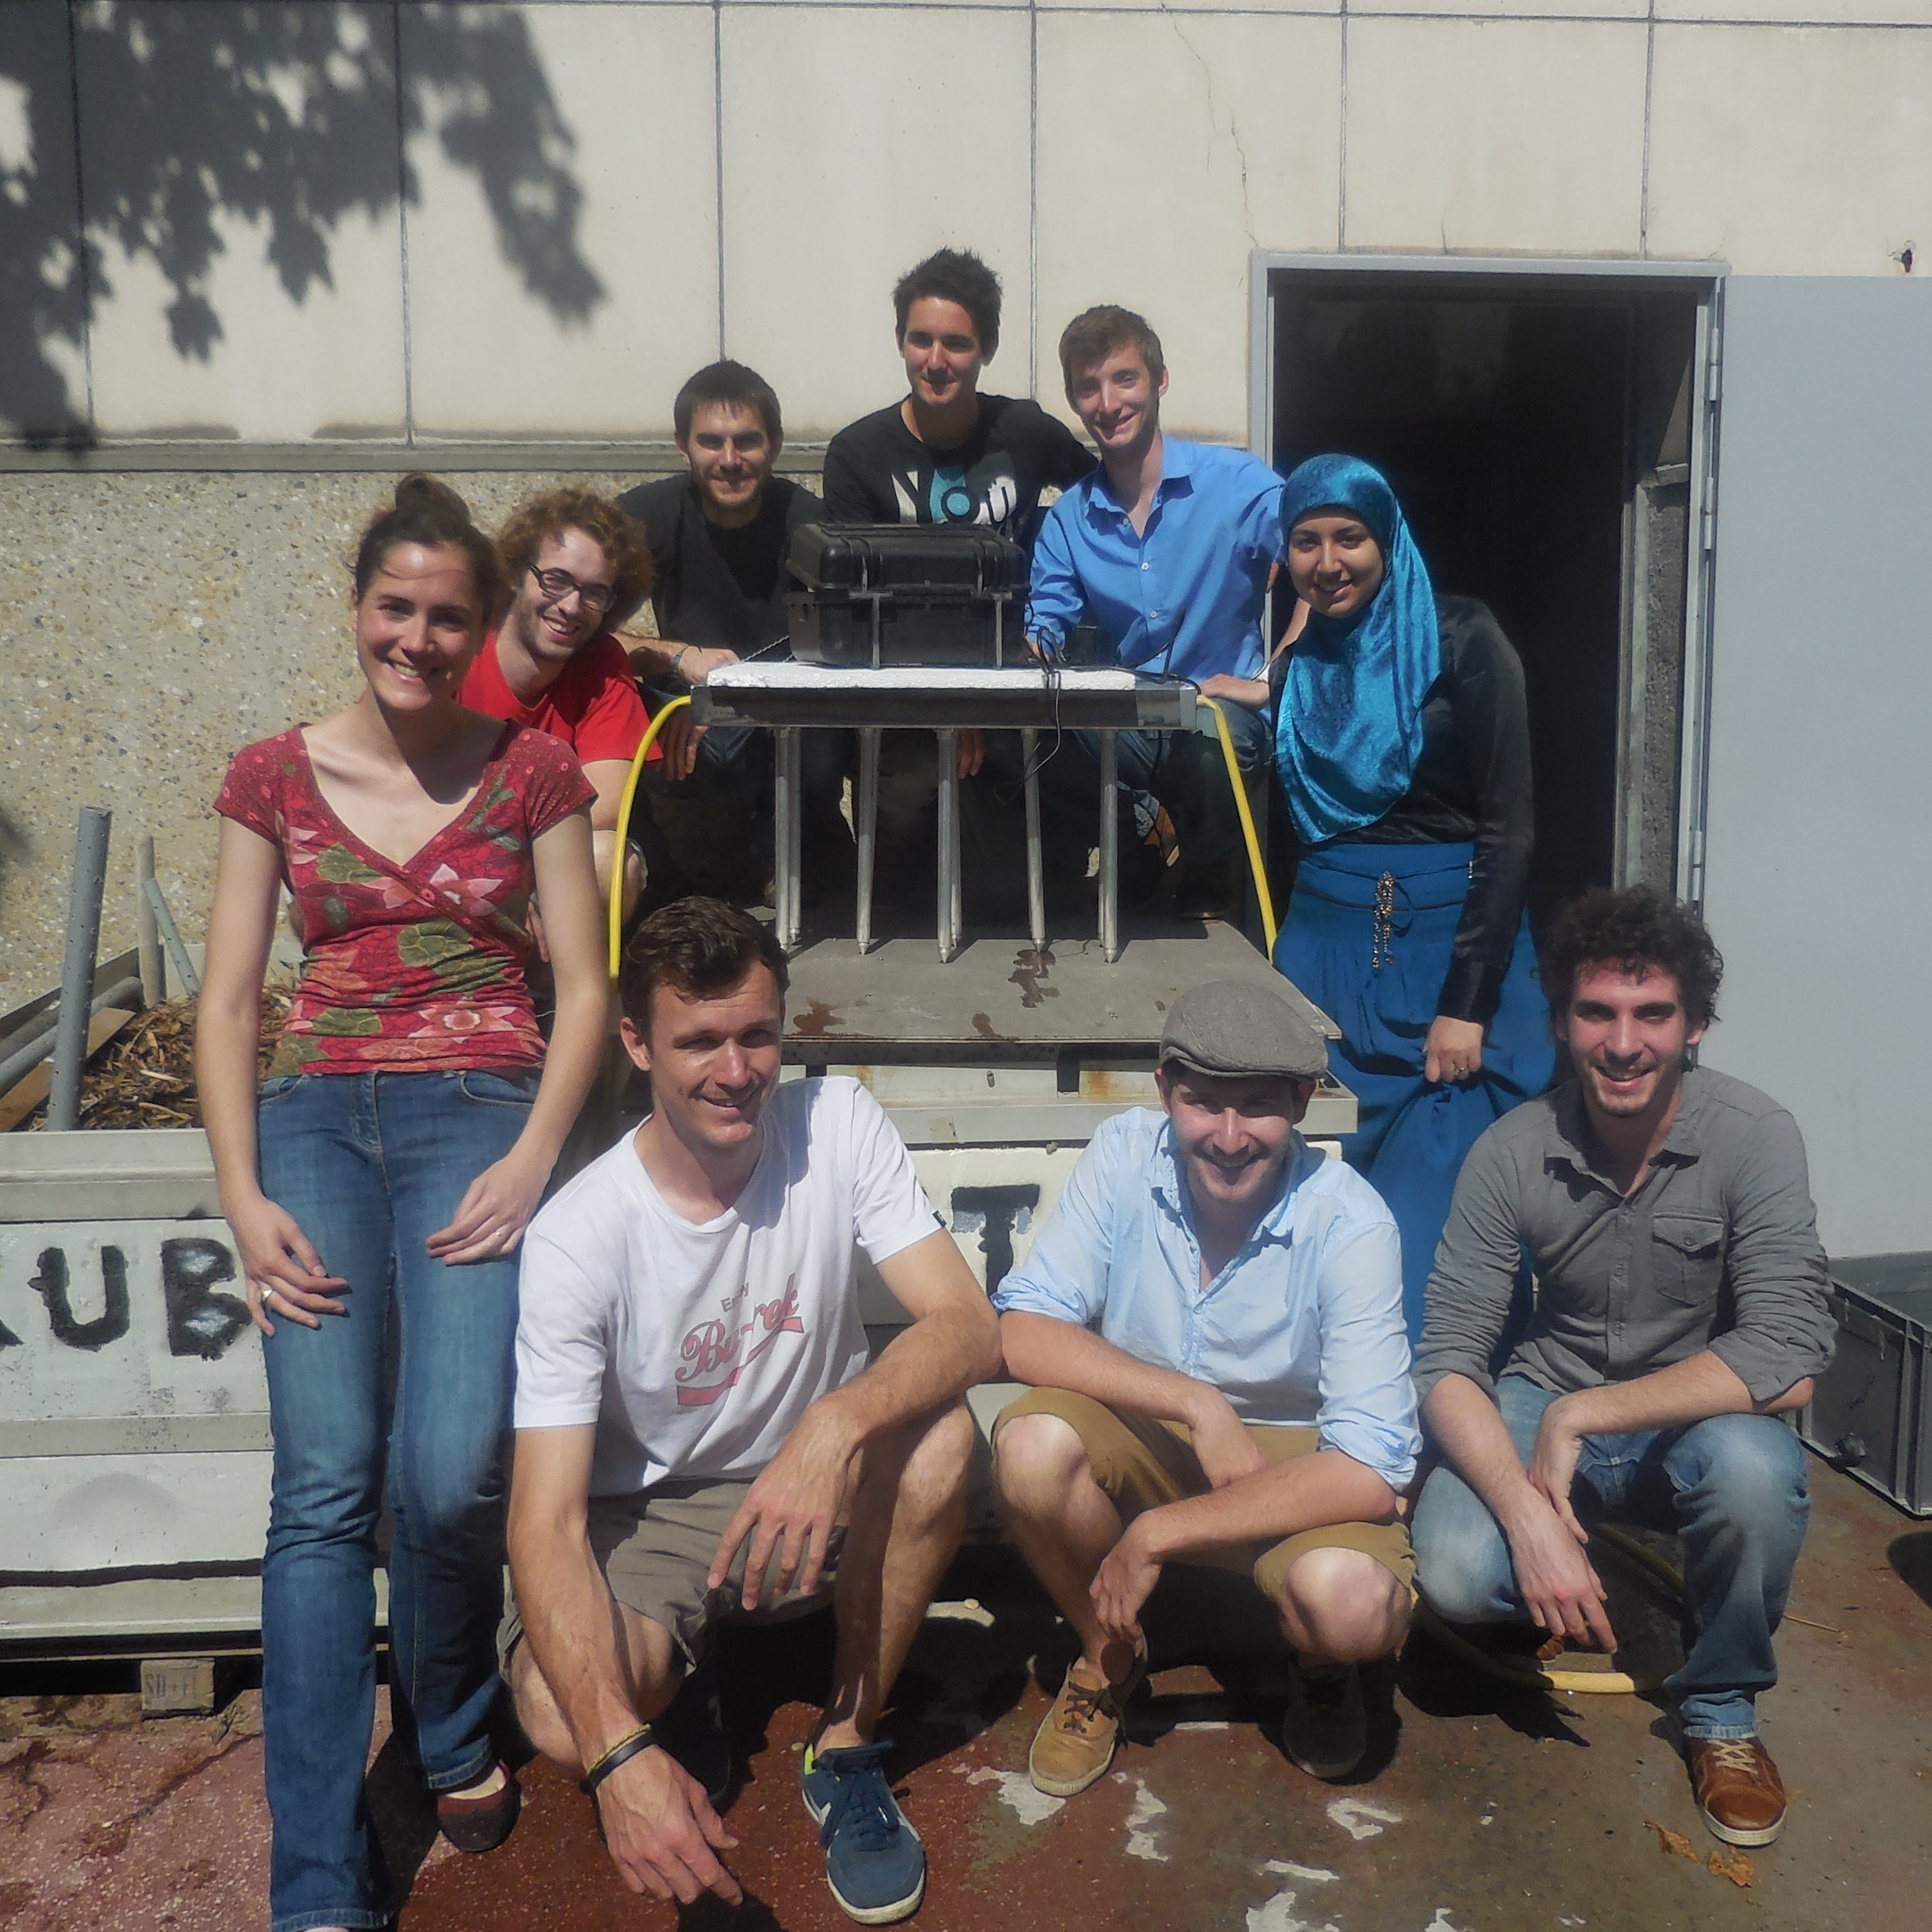
\includegraphics[height=9cm]{/DSCN0447_recadre.JPG}

\par\vspace{\stretch{1}}
   \rule{\linewidth}{.25mm}
\par\textnormal{Soutenu à l'ENS Cachan le 19 Juin 2014}
\par\textnormal{61 avenue du Président Wilson, F-94235 Cachan cedex, France}
\end{center}
%\clearemptydoublepage

\end{document}